\begin{multicols}{3}
	\begin{figure*}
		\subcaptionbox{I punti che voglio raggruppare in 3 gruppi}{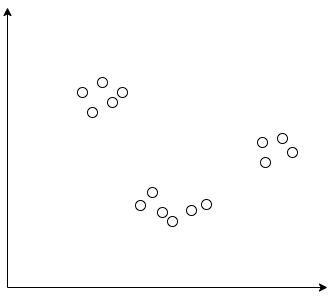
\includegraphics[scale=0.5]{Fase0.png}}\hfill
		\subcaptionbox{Scelti 3 centroidi casualmente}{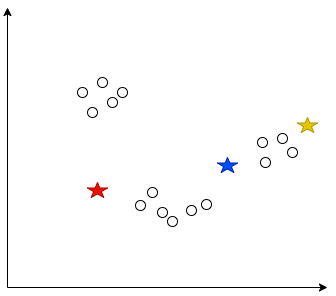
\includegraphics[scale=0.5]{Fase1.png}}\hfill
		\subcaptionbox{Ad ogni osservazione assegno il centroide più vicino in base alla distanza euclidea}{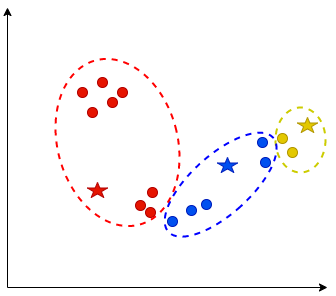
\includegraphics[scale=0.5]{Fase2.png}}\hfill
		\subcaptionbox{Aggiorno i centroidi}{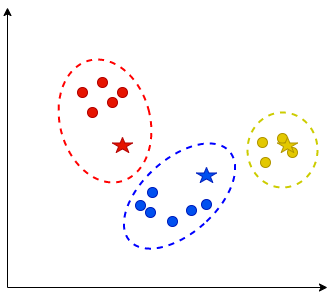
\includegraphics[scale=0.5]{Fase2_bis.png}}\hfill
		\subcaptionbox{Ripeto il punto 2}{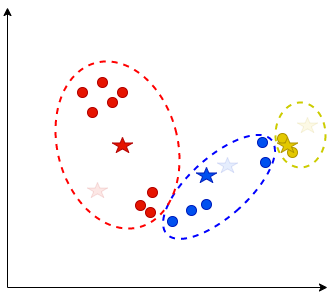
\includegraphics[scale=0.5]{Fase3.png}}
	\end{figure*}
\end{multicols}